% !TEX root = ../main.tex
\section{このフォーマットの使い方}
\label{sec:02-hoge}

\subsection{動作環境}

\TeX{}Live 2018の\upLaTeX{}を使っている.
こういうのはなるべく新しいものを使ったほうがいいぞ.
\upLaTeX{}を使うことで,種﨑敦美みたいな文字を普通に出せるようになる.

\subsection{latexmk}

latexmkrcに必要なことは書いてあるので,latexmkを走らせればpdfが作れる.はず.

\subsection{atom-latex}

Atomのlatexパッケージ\footnote{\url{https://atom.io/packages/latex}}に対応している.
各ファイルの先頭にある\verb|% !TEX|の行は,このパッケージ用のマジックコメントである.

\subsection{ファイル分割}

さすがに大きいと面倒くさそうなのでファイルを分割している.
簡単なのでinputコマンドを使っているが,subfilesなどを利用してもよい.

各ファイルの先頭の\verb|% !TEX root = ../main.tex|のマジックコメントは,書いておくとこのファイルを開いてコンパイルを走らせても勝手にmainがコンパイルされるようにするもの.

\subsection{フォント}
\label{ssec:02-hoge-font}

日本語フォントは各自設定すること.
データも提出するはずなので,フォントの埋め込みは忘れずに.
フォントが埋め込まれているかどうかはAdobeのAcrobatとかでプロパティを見るとわかる.

欧文フォントも日本語に合わせて適当に変えるとよい.
設定するときは\LaTeX Font Catalogue\footnote{\url{http://www.tug.dk/FontCatalogue/}}などを参考にするとよい.

フォントサイズは\verb|documentclass|のオプションで指定する.
指定なし(10pt)にするとPostScript換算で\SI{9.21}{pt}(\SI{9.21}{bp})になってしまって少し小さいので,10ptjを指定して\SI{10}{bp}にしている.

jsclassesでの最新版では,8pt,9pt,10pt,11pt,12pt,14pt,17pt,20pt,21pt,25pt,30pt,36pt,43pt,12Q,14Q,10ptj,10.5ptj,11ptj,12ptjが使える.
\pLaTeX{}での\SI{10}{pt}は\SI{13}{Q}のことで,14Qを指定すると\pLaTeX{}での$10 \times 14/13=\SI{10.77}{pt}$になる.
10ptj(\SI{10}{bp})は,\pLaTeX{}では\SI{10.85}{pt}になる.

\subsection{コマンドの使い方}
\label{ssec:02-hoge-commands}

便利なコマンドをちょこちょこ用意したので使ってほしい.

\subsubsection{数式}

argminやargmaxはコマンドを作ってあるのでそれを使うとよい.
\begin{equation}
    \hat{x} = \argmin_{x} f(x)
    \label{eq:eq1}
\end{equation}

括弧はparen,cbra,sbraコマンドを使うと\verb|\left( \right)|などと同じ処理になる.
\begin{equation}
    i\hbar\diffp*{\psi\paren{\bm{x},t}}{t} = \sbra{\frac{-\hbar^2}{2m}\nabla^2 + V\paren{\bm{x},t}}\psi\paren{\bm{x},t}
    \label{eq:eq2}
\end{equation}
同様にabs,normコマンドもある.
\begin{equation}
    \abs{\jacob{x,y}{r,\theta}} = r
    \label{eq:eq3}
\end{equation}
\begin{equation}
    \norm{A}_F = \sqrt{\sum_{i=1}^m\sum_{j=1}^n\abs{a_{ij}}^2}
    \label{eq:eq4}
\end{equation}

条件付き確率を書くためだけのagivenbとagivenbpコマンドもある.
pが付いている方は括弧もついでに書く.
\begin{equation}
    p\agivenbp{\bm{x}}{\bm{\alpha}} = \frac{\Gamma\paren{\prod^P\alpha_p}}{\prod_p^P\Gamma\paren{\alpha_p}}\prod_p^Px_p^{\alpha_p-1}
    \label{eq:eq5}
\end{equation}

偏微分はdiffcoeffパッケージを使っている.
diffcoeffでググると僕の記事が上の方に出てくるので使うとよい.

\begin{equation}
    \kappa_n = \diff[n]{K_X(t)}{t}[t=0] = \begin{cases}
        \mu+\gamma\eta & (n=1) \\
        \eta^k(n-1)!\zeta(n) & (n \geq 2)
    \end{cases}
    \label{eq:eq6}
\end{equation}

\subsubsection{文字の強調}

enhanceコマンドで文字列が\enhance{このようにゴシック体になってstrongになる}ようになっている.
名前がstrongじゃないのはなんか他のパッケージとぶつかるからだった気がする.

\subsubsection{URL}

urlパッケージをデフォルトで読み込んである。urlコマンドでURLがなんかいい感じに出力される.

\subsubsection{subfigure}

2つ画像を並べるときがときどきあるので,それ用のコマンドを用意してある.
\ref{fig:yayoiori}にその例を示す.

\twofigure{
    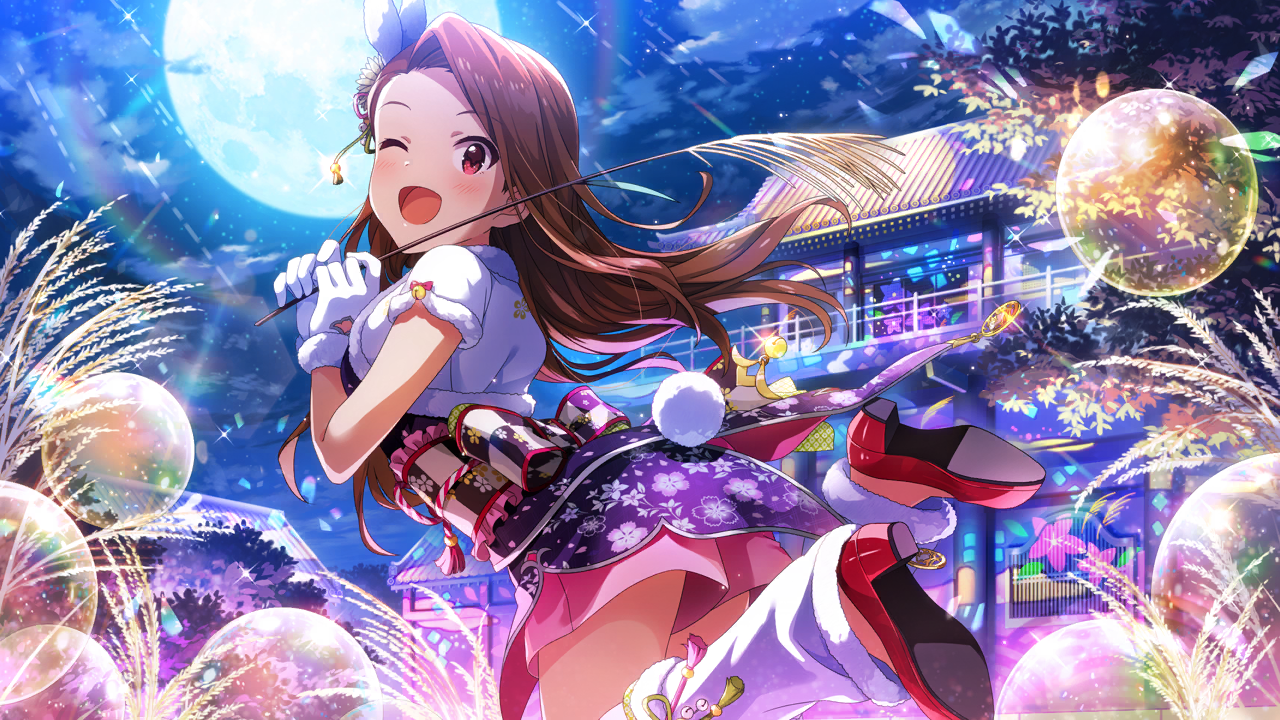
\includegraphics[width=.8\linewidth]{007ior0084_1.png}
    \subcaption{水瀬伊織}
    \label{fig:iori}
}{
    
\includegraphics[width=.8\linewidth]{005yay0084_1.png}
    \subcaption{高槻やよい}
    \label{fig:yayoi}
}{
    \caption[フェス限の伊織とやよいの比較]{フェス限の伊織とやよいの比較(ともに特訓後).どっちもかわいい.}
    \label{fig:yayoiori}
}

\subsection{参照}

あらゆる参照はrefコマンドだけでOKなようになっている.
「図」とか「表」とか「節」とか「式」とかは空気を読んで勝手に入る.

\ref{fig:kana}に特訓前のフェス限矢吹可奈の画像を示す.
また,最近のフェス限の性能比較は\ref{tbl:fes}に示す.

\begin{figure}
    \centering
    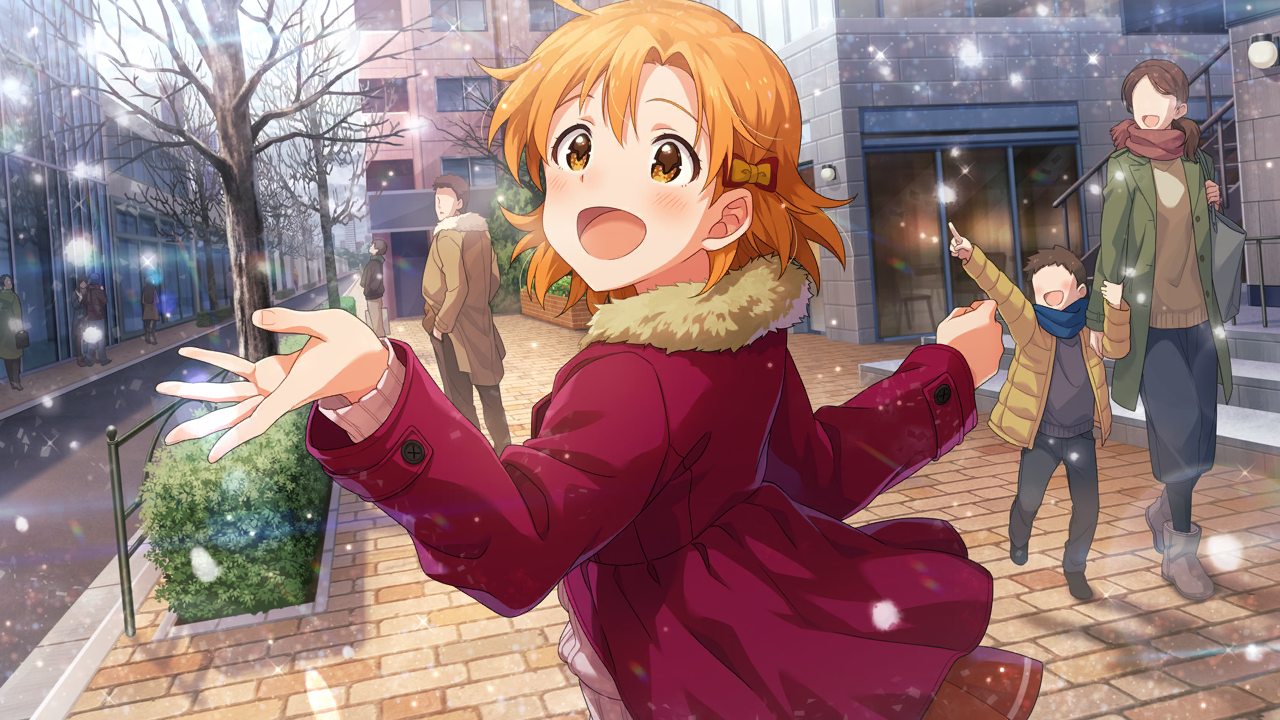
\includegraphics[width=.8\linewidth]{036kan0104_0.png}
    \caption[フェス限矢吹可奈]{フェス限矢吹可奈(特訓前).雪ではしゃぐ矢吹可奈はかわいい.}
    \label{fig:kana}
\end{figure}

\begin{table}
    \centering
    \caption[フェス限やよいおりとかなしほの性能比較]{フェス限やよいおりとかなしほの性能比較(すべて特訓後☆4時).センターに配置すると,特化値が+95\%されることに留意する.こう見ると伊織が結構弱い.}
    \begin{tabular}{cc|cccc|crcc}
        \toprule
        アイドル & タイプ & Vo & Da  & Vi & 合計 & 特技 & 間隔 & 確率 & 時間 \\ \hline\hline
        矢吹可奈 & Princess & 6433 & 3272 & 9630 & 19335 & \multirow{4}{*}{コンボナ28\%} & 7秒 & \multirow{4}{*}{40\%} & 4秒 \\\cline{1-6}\cline{8-8}\cline{10-10}
        北沢志保 & \multirow{2}{*}{Fairy} & 3262 & \textbf{9631} & 6454 & \textbf{19347} & & 13秒 & & 7秒 \\\cline{1-1}\cline{3-6}\cline{8-8}\cline{10-10}
        水瀬伊織 &  & 6452 & 9578 & 3216 & 19246 & & 11秒 & & 6秒 \\\cline{1-6}\cline{8-8}\cline{10-10}
        高槻やよい & Angel & 9601 & 6446 & 3280 & 19327 & & 10秒 & & 5秒\\
        \bottomrule
    \end{tabular}
    \label{tbl:fes}
\end{table}

章や節の参照は\ref{sec:02-hoge}とか\ref{ssec:02-hoge-font}とかになる.

refはcleverefを使っているので,\verb|\ref{eq:eq1,eq:eq2,eq:eq3}|などとカンマ区切りで使える.
使うと\ref{eq:eq1,eq:eq2,eq:eq3,eq:eq5}のように勝手にいい感じになる.
なお,章と節の参照をカンマ区切りで指定するとおかしくなっちゃうので,これは使わないほうがよい(設定するのが面倒くさかった).

\subsection{参考文献}

参考文献と発表文献を分けて書けるようになっている.
普通にciteすると参考文献に載るようになっており,発表文献のファイルはデフォルトですべて出力されるようになっている.
発表文献の順序はbibファイルに書かれている順序になる.

\subsection{脚注}

デフォルトの脚注のデザインがあまり好きじゃないのでいじってある.

\begin{center}
    \begin{minipage}{0.6\linewidth}
        \LaTeX{}では,minipage環境内で別の脚注を使うことができる.
        このテンプレートはそれにも対応している\footnote{こんな感じ.}.
        mpfootnotemarkコマンドをjsclasses用に作り変えたやつを定義してあるので,こんな感じに使える\mpfootnotemark[765].
        \footnotetext[765]{765個も脚注はない.}
    \end{minipage}
\end{center}
